\section{Ternary Mixtures}

The pseudo-analytical approach for ternary mixtures in table \ref{TernarySystemsandReferences}, as discussed in section \ref{TernaryPAMethodSection}, was applied for the DWPM model using the Python programming language. These results are now presented. As before, $s_{1}$ through $s_{3}$ are arbitrarily chosen as $\nicefrac{1}{2}$, thereby reducing the DWPM model to a modified form of the Wilson model. In the case of ternary mixtures which exhibit only one two-phase region, this form of the model was found to be adequate to match the experimental measurements. The software was however created to accommodate variable values for each $s_{i}$. The results for the system 1-Hexanol, Nitro-Methane and Water indicate that this might be necessary to model systems which have more complex phase diagrams.\\

%% Cyclohexane-Benzene-Methanenitro--------------------------------------------------------------------------------%

The experimentally measured composition points for the mixture Cyclohexane, Benzene and Nitro-Methane, at $298.15~\mathrm{K}$, are given in table \ref{TielineDatacyclohexane-benzene-methanenitro}. The binary interaction parameters, reported in table \ref{TernaryParameterResultsTable}, were calculated using the first and third experimentally measured tie-lines in table \ref{TielineDatacyclohexane-benzene-methanenitro}. The position of the tie-lines used for the calculation and the shape of the resulting Gibbs energy surface is illustrated in figure \ref{cyclohexane-benzene-methanenitroGibbsEnergySurface}. The region where the Hessian matrix of the Gibbs energy function in figure \ref{cyclohexane-benzene-methanenitroGibbsEnergySurface} is not positive definite, i.~e. where the mixture is unstable, is indicated by the red projection below the Gibbs energy surface.\\ 

\begin{table}[h]
\caption{Experimental tie-line data for the system Cyclohexane, Benzene and Nitro-Methane at $298.15~\mathrm{K}$}
\centering
\begin{tabular}{cccc}
\toprule
\multicolumn{2}{c}{\textbf{Phase 1}} & \multicolumn{2}{c}{\textbf{Phase 2}}\\
$x_{1}$& $x_{2}$ &$x_{1}$& $x_{2}$\\
\midrule
0.820 & 0.117 & 0.047 & 0.035\\
0.721 & 0.189 & 0.070 & 0.099\\
0.563 & 0.263 & 0.094 & 0.147\\
\bottomrule
\end{tabular}\\
\label{TielineDatacyclohexane-benzene-methanenitro}
\end{table}

\begin{landscape}
\vspace*{\fill}
\begin{table}[h]
\caption{Binary interaction parameters calculated form ternary tie-line data}
\centering
\begin{tabular}{ccccccc}
\toprule
\textbf{Temperature}/$\mathrm{K}$&$\Lambda_{12}$&$\Lambda_{21}$&$\Lambda_{13}$&$\Lambda_{31}$&$\Lambda_{23}$&$\Lambda_{32}$\\
\midrule
\multicolumn{7}{l}{\textbf{Cyclohexane, Benzene and Nitro-Methane}}\\
\midrule
\textbf{ 298.15 } & \num{3.386d-2} & \num{2.208} & \num{1.145d-1} & \num{7.717d-2} & \num{5.723d-2} & \num{1.445}\\
\midrule
\multicolumn{7}{l}{\textbf{Heptane, Hexane and Methanol}}\\
\midrule
\multicolumn{7}{l}{\emph{From the third and fourth experimentally measured tie-lines}}\\
\textbf{ 305.95 } & \num{2.163d-2} & \num{5.027} & \num{1.488d-1} & \num{3.565d-1} & \num{1.592d-1} & \num{2.610d-1}\\
\multicolumn{7}{l}{\emph{From the third and second last experimentally measured tie-lines}}\\
\textbf{ 305.95 } & \num{1.990d-1} & \num{5.136} & \num{1.849d-1} & \num{2.760d-01} & \num{2.026d-1} & \num{4.009d-1}\\
\midrule
\multicolumn{7}{l}{\textbf{1-Hexanol, Nitro-Methane and Water}}\\
\midrule
\textbf{ 294.15 } & \num{9.434d-2} & \num{7.628d-1} & \num{3.236d-4} & \num{1.761} & \num{6.487d-2} & \num{2.983d-1}\\
\textbf{ 296.15 } & \num{9.412d-2} & \num{7.386d-1} & \num{3.099d-4} & \num{1.753} & \num{6.476d-2} & \num{3.099d-1}\\
\bottomrule
\end{tabular}\\
\label{TernaryParameterResultsTable}
\end{table}
\vspace*{\fill}
\end{landscape}

\begin{figure}[h]
\vspace{40pt}
\centering
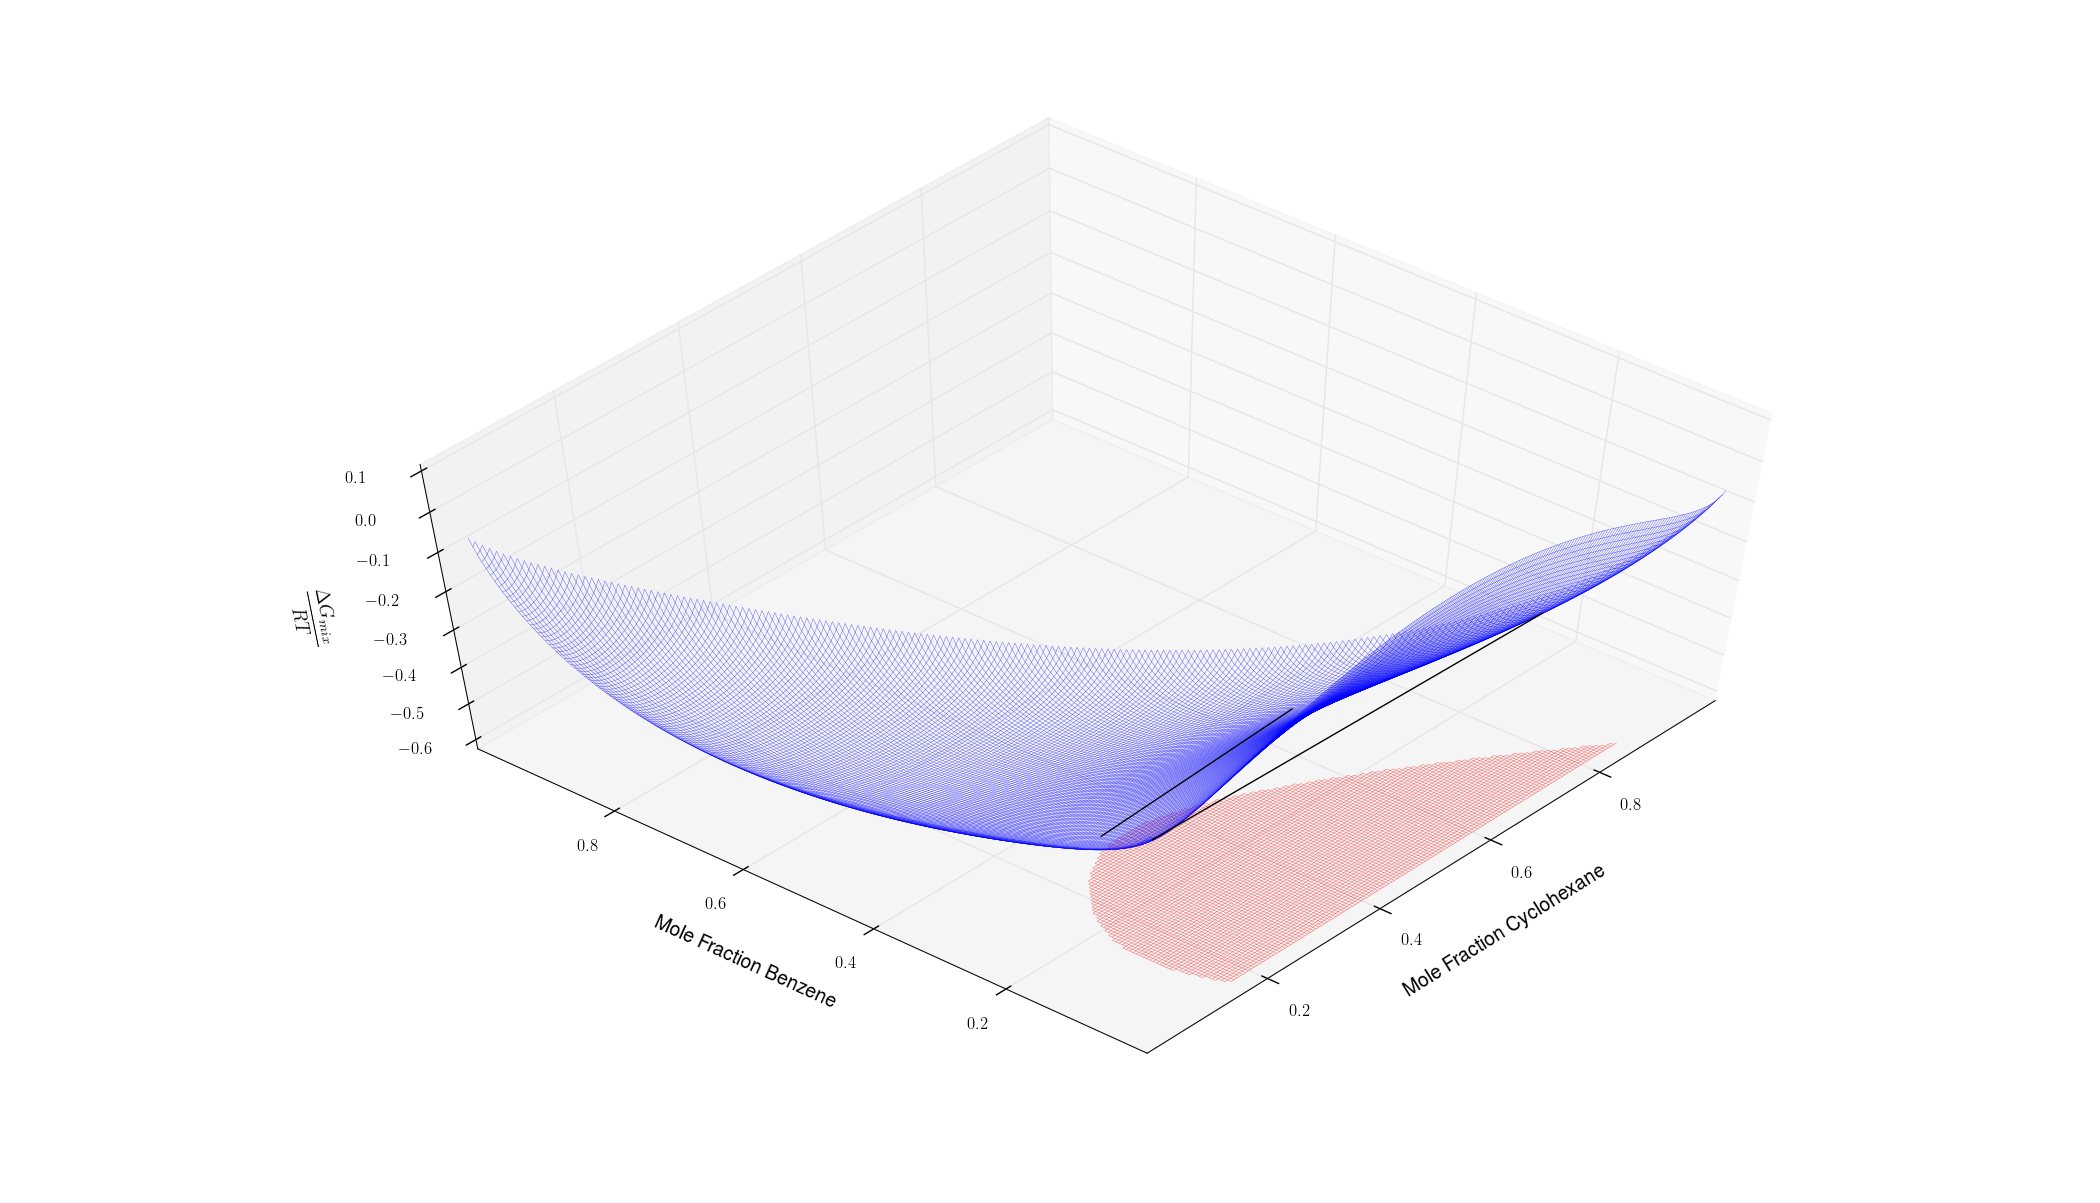
\includegraphics[width = \textwidth, bb=100 100 1600 700]{Results_Parts/TernaryParams/cyclohexane-benzene-methanenitro/DWPM/rotation1.png}
\caption{Predicted Gibbs energy surface for Cyclohexane, Benzene and Nitro-Methane at $298.15~\mathrm{K}$}
\label{cyclohexane-benzene-methanenitroGibbsEnergySurface}
\end{figure}	

Figure \ref{cyclohexane-benzene-methanenitroFigure} shows the predicted ternary phase diagram, calculated with the method discussed in section \ref{TernaryPAMethodSection}. From figure \ref{cyclohexane-benzene-methanenitroFigure} it is clear that the calculated parameters predict a phase envelope which matches the experimental data very well. Unlike in the case of the binary mixtures studied, which have experimental data for only one tie-line at a given temperature, experimental measurements for multiple tie-lines may be available for ternary mixtures. Seeing as the pseudo analytical approach utilises only two of theses tie-lines at a time, available experimental data points which are not included in this calculation will not be reproduced exactly. There is therefore a choice of which tie-lines to utilise for parameter estimation, and in this case they were chosen arbitrarily. In cases where experimental data for multiple tie-lines are available, statistical methods may be used to determine a set of parameters which best fit all experimental data points. In other words, a method like the principle of maximum likelihood for example, may be used to determine the set of tie-lines whose use together with the pseudo-analytical approach, yield the best overall fit to experimental data. Although no statistical analysis was performed in this investigation, it could be applied in future investigations.\\

\begin{figure}[h]
\centering
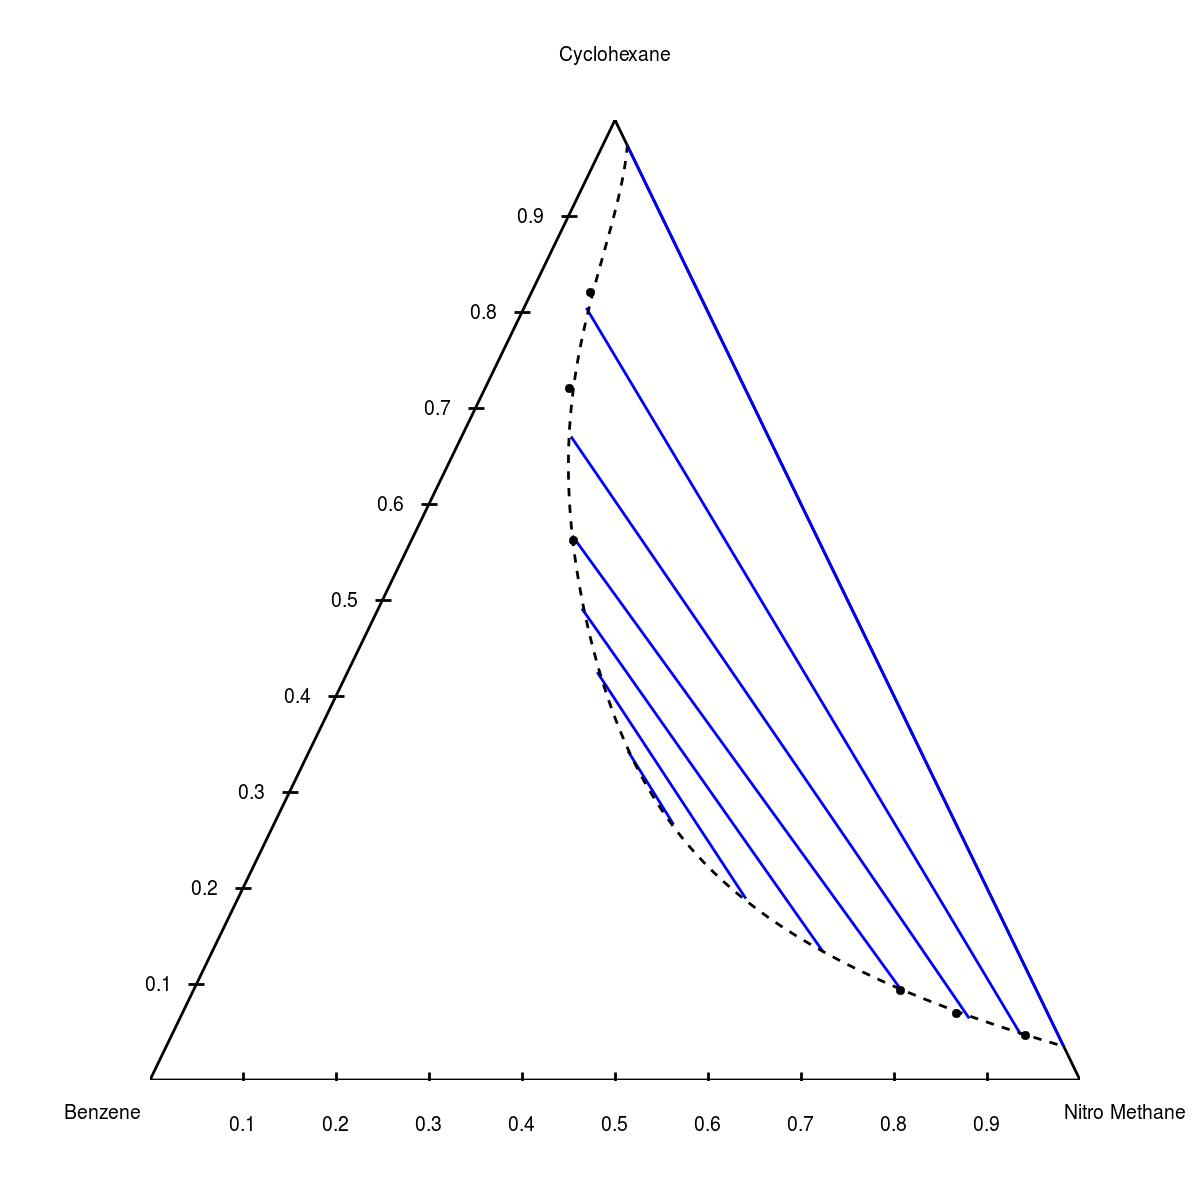
\includegraphics[width = 0.85\textwidth, bb=50 50 900 900]{Results_Parts/TernaryParams/cyclohexane-benzene-methanenitro/DWPM/CalculatedPhaseDiagram.png}
\caption{Calculated ternary phase diagram for Cyclohexane, Benzene and Nitro-Methane at $298.15~\mathrm{K}$} \label{cyclohexane-benzene-methanenitroFigure}
\end{figure}	
\clearpage
%% Heptane-Hexane-Methanol-----------------------------------------------------------------------------------------%

This aforementioned principle is illustrated well by the results for the system Heptane, Hexane and Methanol. For this system, the equilibrium compositions for a number of tie-lines have been measured at $305.95~\mathrm{K}$. This experimental tie-line data is given in tale \ref{TielineDataheptane-hexane-methanol}. The model parameters calculated using the information from the third and fourth experimentally measured tie-lines are given in table \ref{TernaryParameterResultsTable}. The position of the tie-lines used for the parameter calculation and the Gibbs energy surface is shown in figure \ref{heptane-hexane-methanolGibbsEnergySurface1}.\\

\begin{table}[h]
\caption{Experimental tie-line data for the system Heptane, Hexane and Methanol at  $305.95~\mathrm{K}$ }
\centering
\begin{tabular}{cccc}
\toprule
\multicolumn{2}{c}{\textbf{Phase 1}} & \multicolumn{2}{c}{\textbf{Phase 2}}\\
$x_{1}$& $x_{2}$ &$x_{1}$& $x_{2}$\\
\midrule
0.806 & 0.000 & 0.130 & 0.000\\
0.625 & 0.147 & 0.110 & 0.023\\
0.522 & 0.227 & 0.104 & 0.049\\
0.416 & 0.330 & 0.091 & 0.077\\
0.261 & 0.459 & 0.060 & 0.132\\
0.184 & 0.538 & 0.041 & 0.155\\
0.166 & 0.544 & 0.045 & 0.166\\
0.061 & 0.582 & 0.018 & 0.229\\
0.000 & 0.626 & 0.000 & 0.296\\
\bottomrule
\end{tabular}\\
\label{TielineDataheptane-hexane-methanol}
\end{table}

\begin{figure}[h]
\vspace{40pt}
\centering
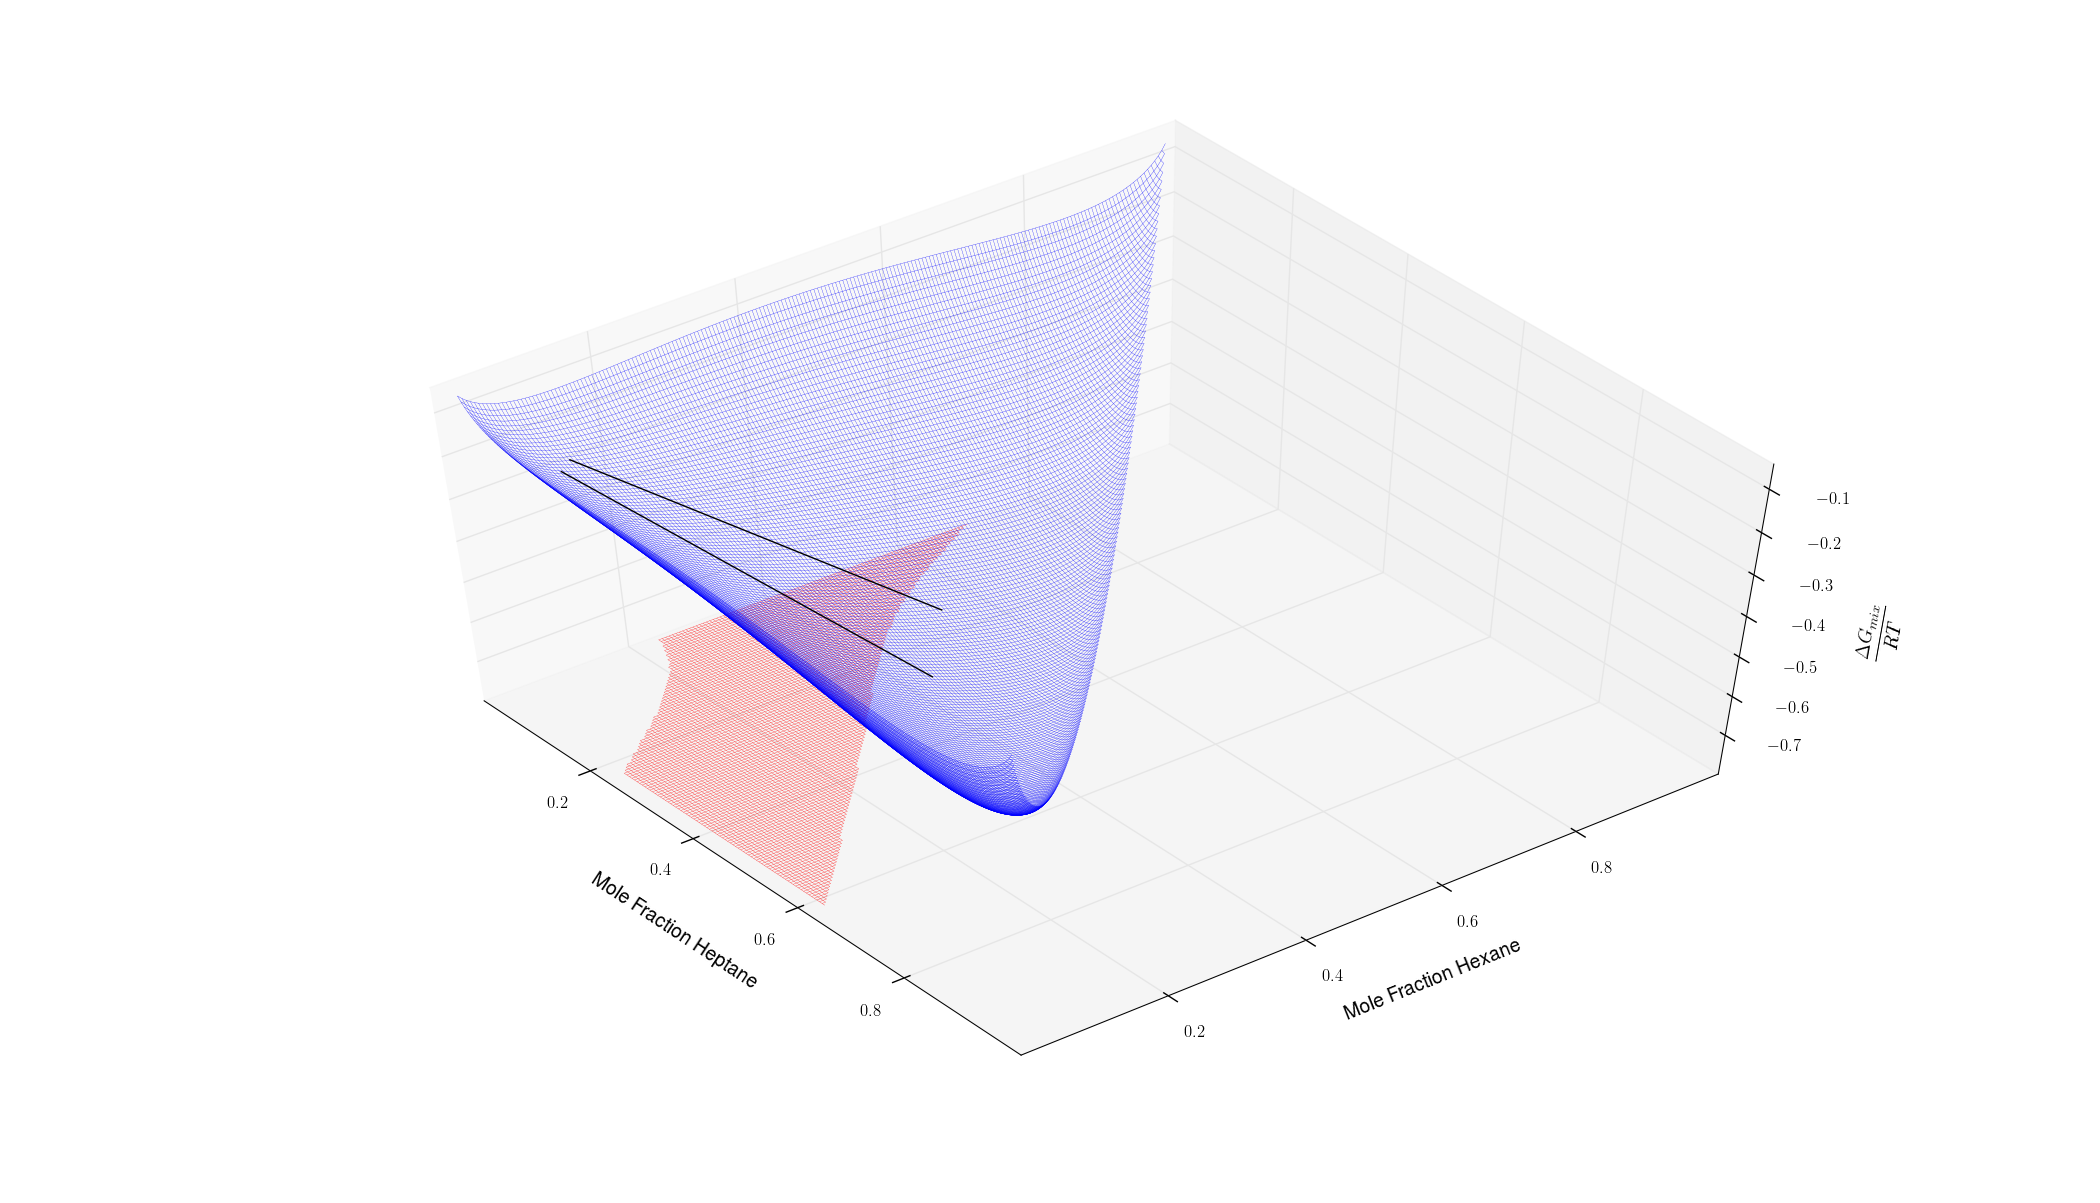
\includegraphics[width = \textwidth, bb=100 100 1600 700]{Results_Parts/TernaryParams/heptane-hexane-methanol/DWPMTieline3and4/rotation3.png}
\caption{Predicted Gibbs energy surface for Heptane, Hexane and Methanol at $305.95~\mathrm{K}$, using parameters calculated from experimental tie-lines 3 and 4.}
\label{heptane-hexane-methanolGibbsEnergySurface1}
\end{figure}

From the phase diagram in figure \ref{heptane-hexane-methanolFigure1}, it is observed that these parameters match the experimental tie-line data well in the region of the data used for the parameter estimation. As the fraction of Heptane decreases however, and the binary mixture of Hexane and Methanol is approached, the shape of the two-phase region clearly does not correspond well to the experimental data.\\

\begin{figure}[h]
\centering
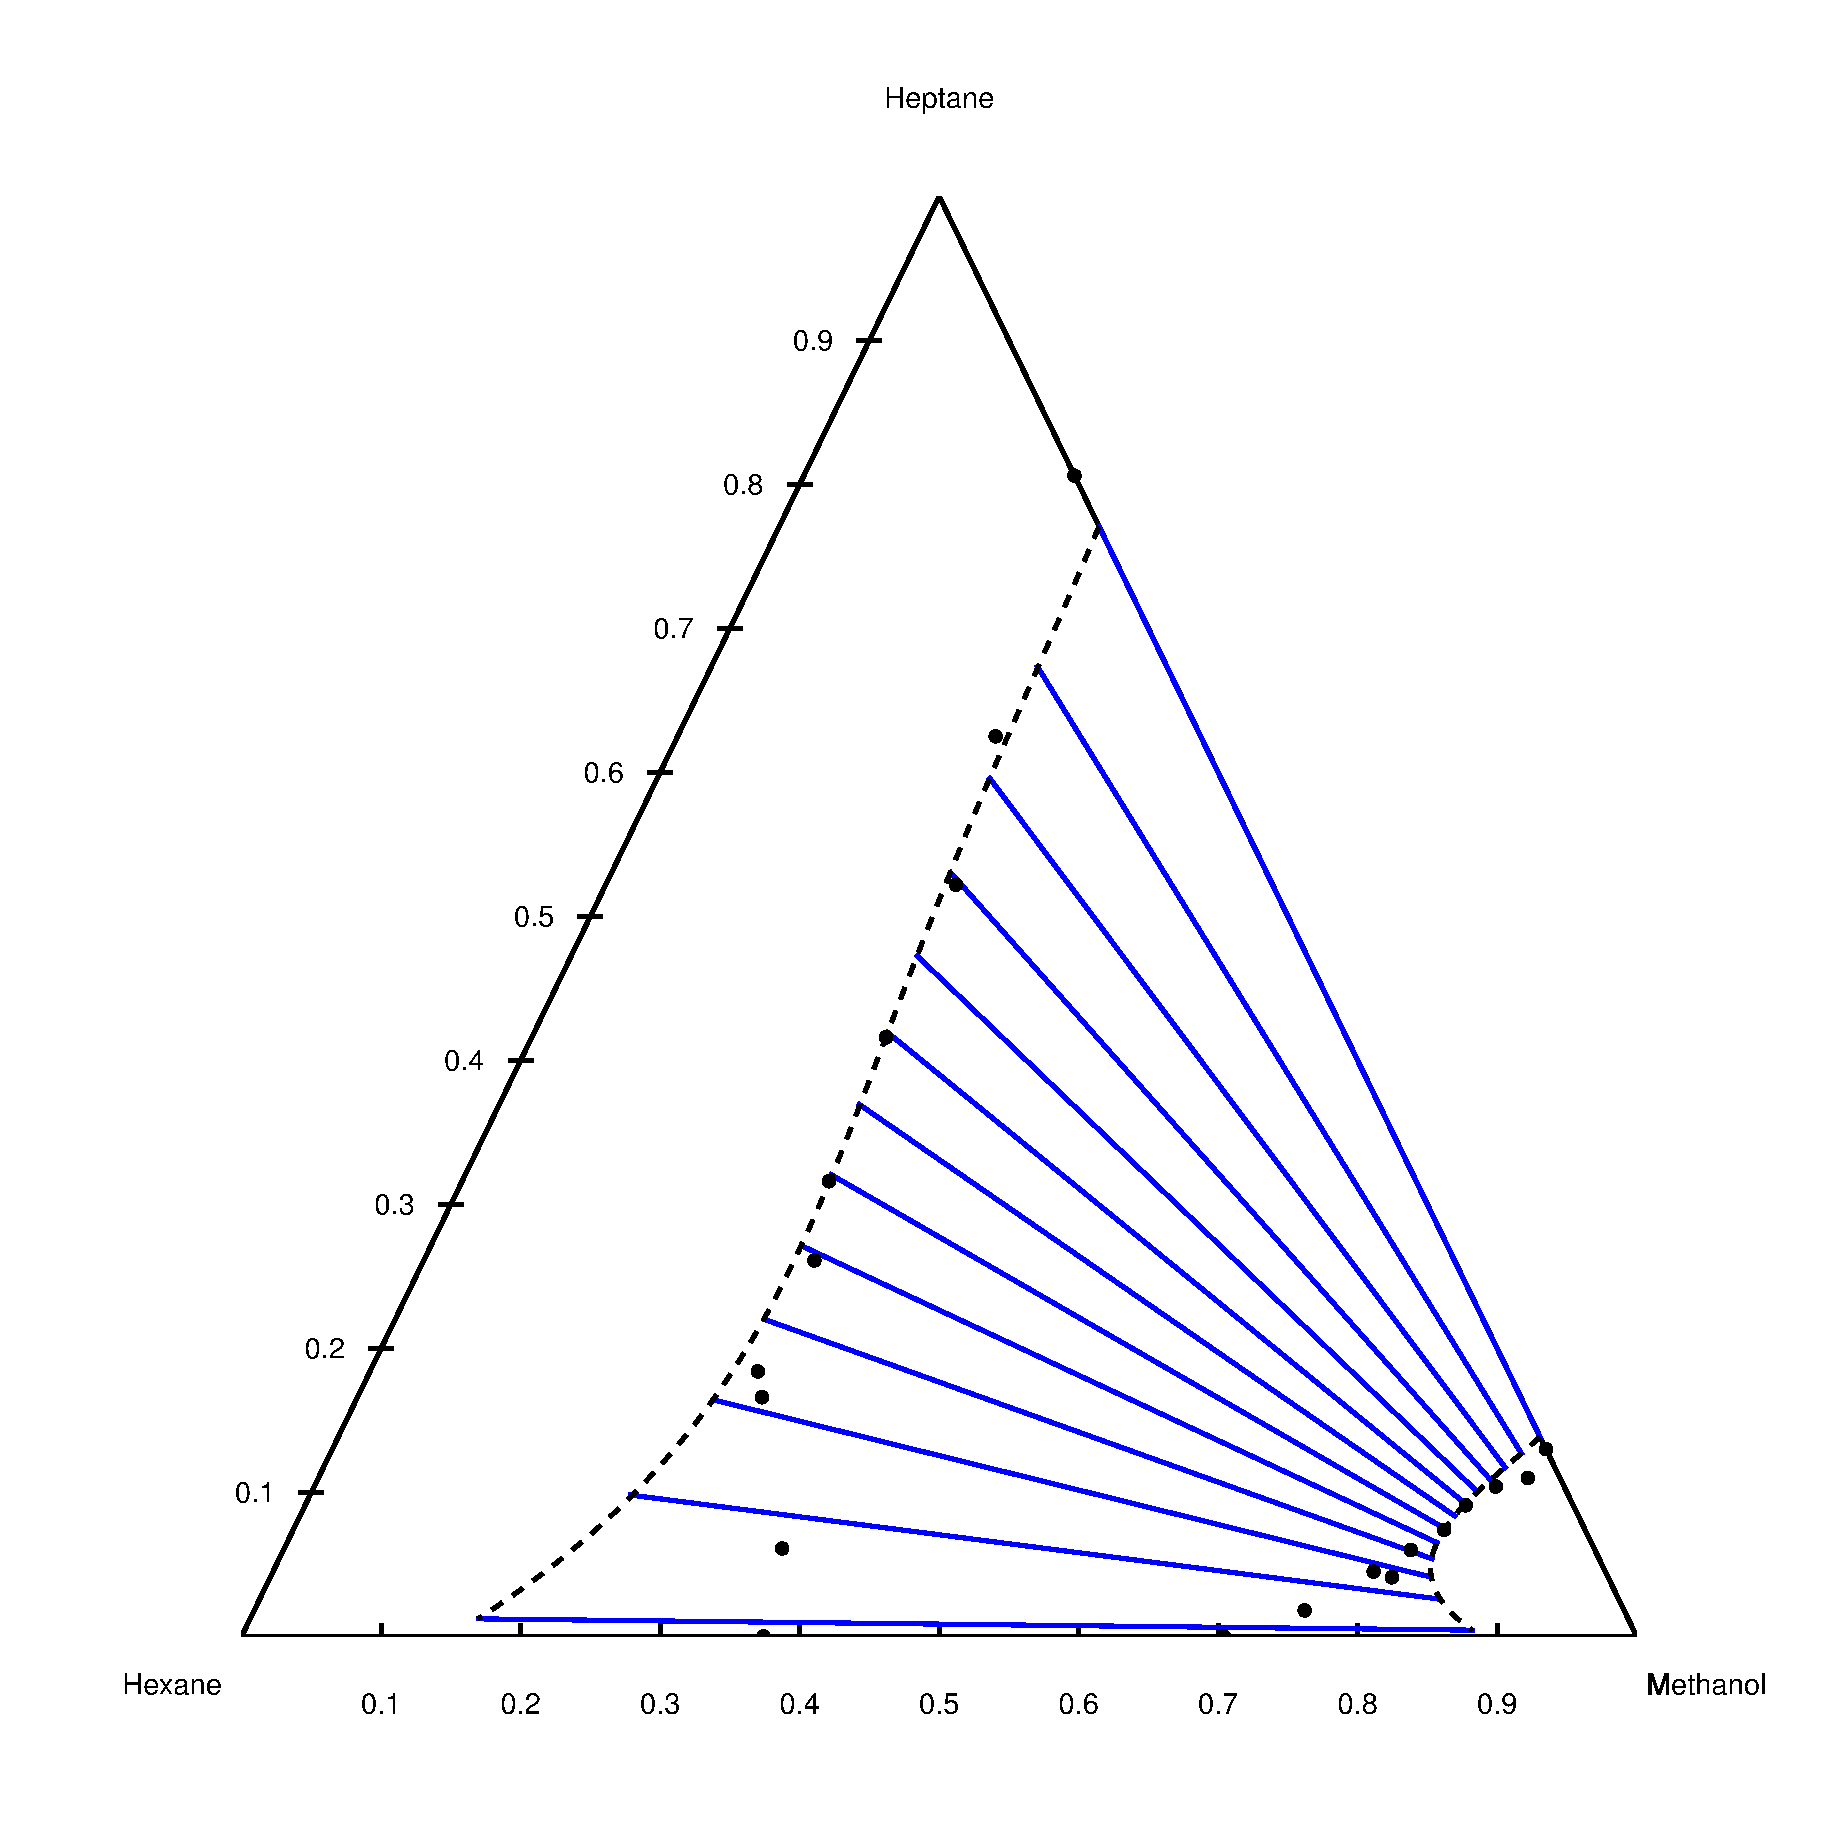
\includegraphics[width = 0.85\textwidth]{Results_Parts/TernaryParams/heptane-hexane-methanol/DWPMTieline3and4/CalculatedPhaseDiagram.eps}
\caption{Calculated ternary phase diagram for Heptane, Hexane and Methanol, using the parameters calculated from the third and fourth experimentally measured tielines} \label{heptane-hexane-methanolFigure1}
\end{figure}	
\clearpage

From figure \ref{heptane-hexane-methanolGibbsEnergySurface1}, considering the size of the two phase-region, it seems that the experimental tie-lines used for the parameter calculation are situated relatively close together. In an attempt to better match the experimental data of the entire phase diagram, the model parameters were recalculated using data from tie-lines which are spaced further apart. The resulting parameters, calculated using the third and second last experimentally measured tie-lines, are given in table \ref{TernaryParameterResultsTable}. The tie-lines and resulting Gibbs energy surface for this instance is shown in figure \ref{heptane-hexane-methanolGibbsEnergySurface2}.\\

\begin{figure}[h]
\vspace{40pt}
\centering
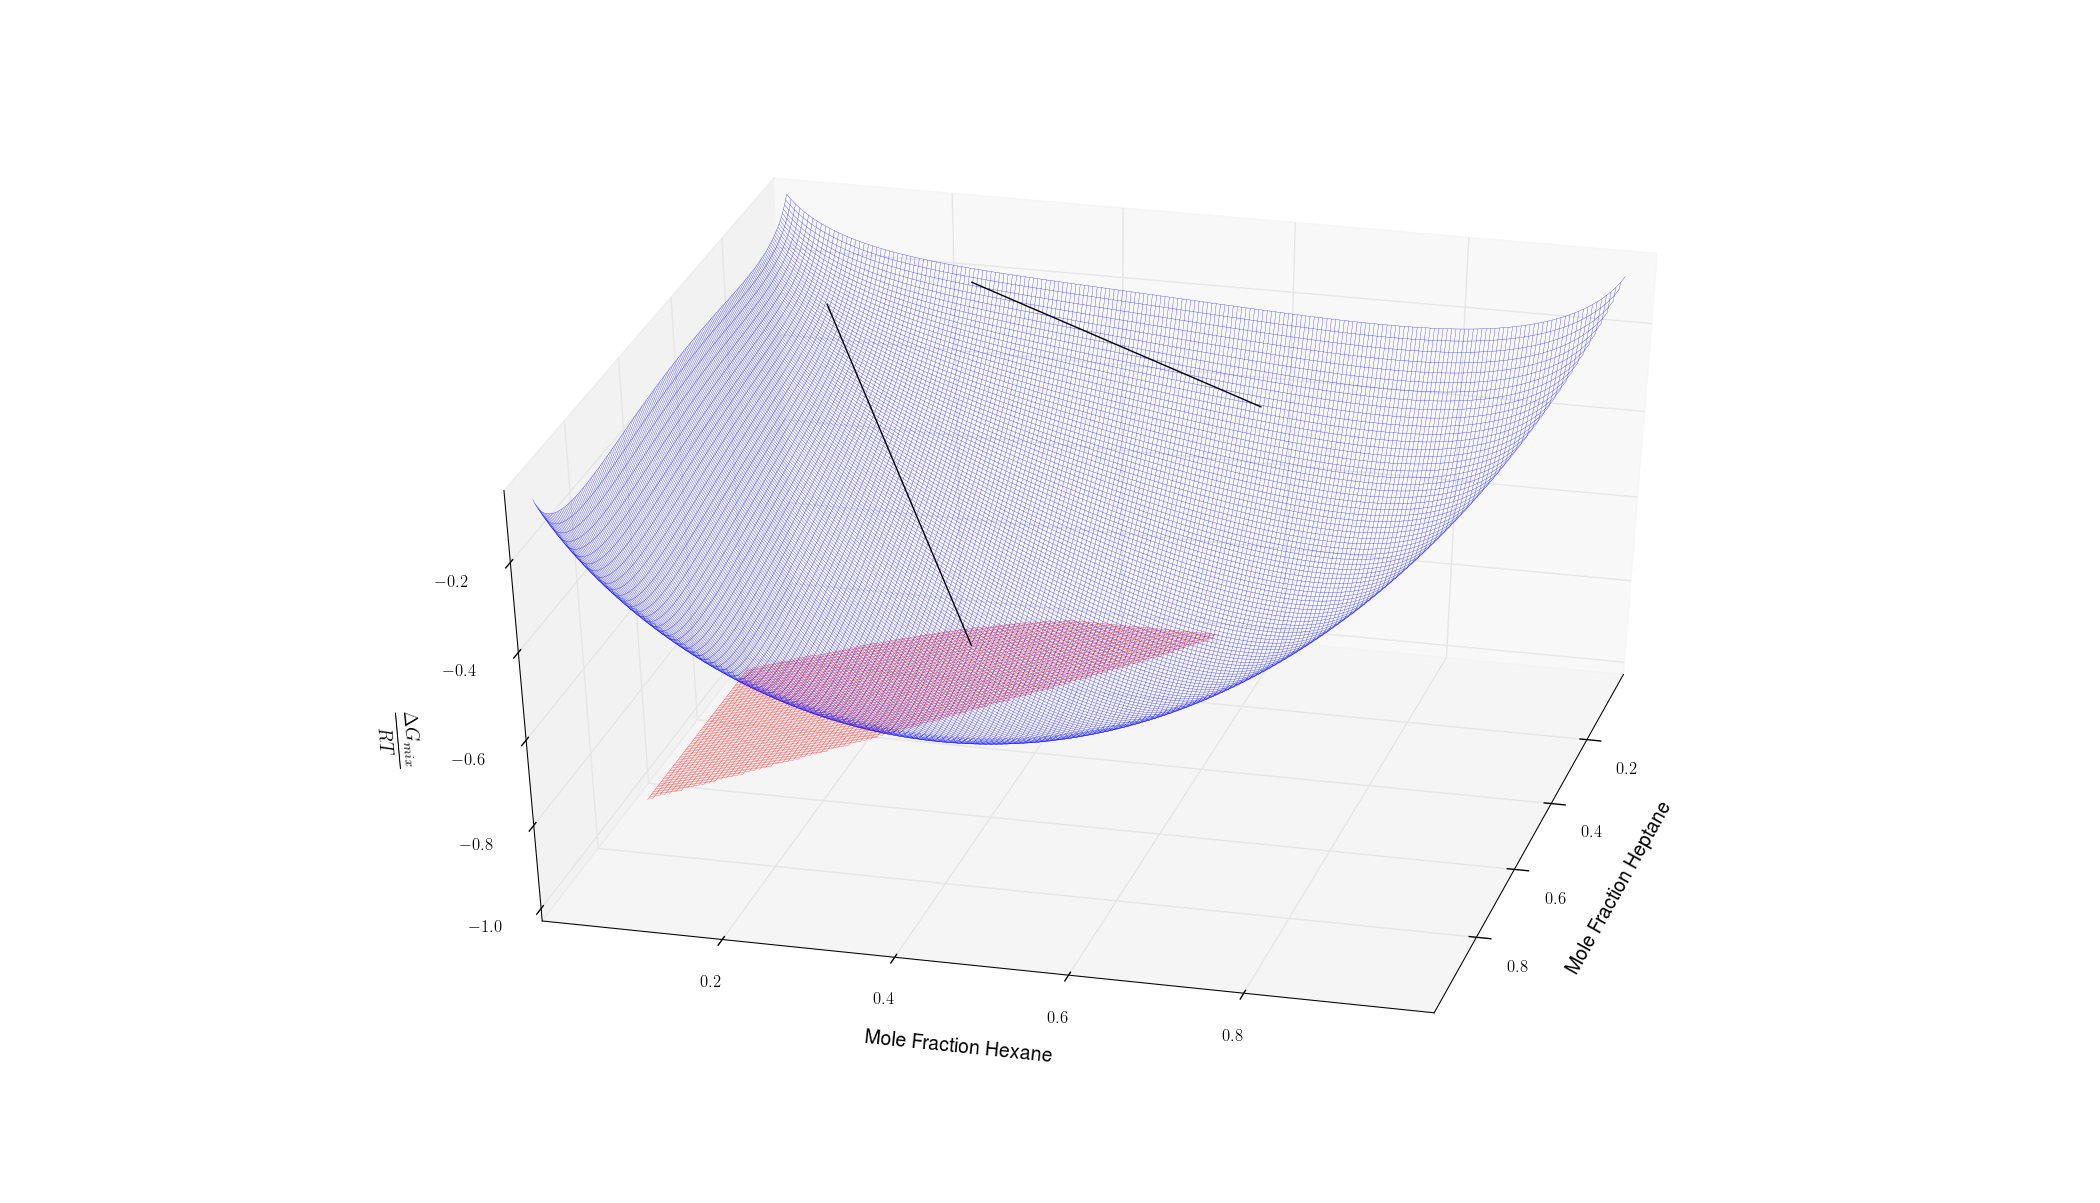
\includegraphics[width = \textwidth, bb=100 100 1600 700]{Results_Parts/TernaryParams/heptane-hexane-methanol/DWPMTieline3and-2/rotation6.png}
\caption{Predicted Gibbs energy surface for Heptane, Hexane and Methanol at $305.95~\mathrm{K}$, using parameters calculated from experimental tie-lines 3 and second to last.}
\label{heptane-hexane-methanolGibbsEnergySurface2}
\end{figure}	

The phase diagram resulting from the newly calculated binary parameters, in figure \ref{heptane-hexane-methanolFigure2}, shows a marked improvement in the shape of the two-phase region. The binary phase splits are also apparently reproduced more accurately than in figure \ref{heptane-hexane-methanolFigure1}.\\

No statistical method was applied here to determine a set of parameters which most accurately reproduce all the experimental data points. The choice of tie-lines used for the parameter estimation was made arbitrarily. By inspection of the resulting phase diagrams, the interaction parameters calculated using the third and second to last measured tie-lines were deemed more suitable.\\

From the ternary phase diagram, it is also clear that random and/or experimental errors are present in the experimental data. While it was not done here, the availability of a relatively large number of experimental data points enables the application of a statistical method to smooth the experimental data.\\

\begin{figure}[h]
\centering
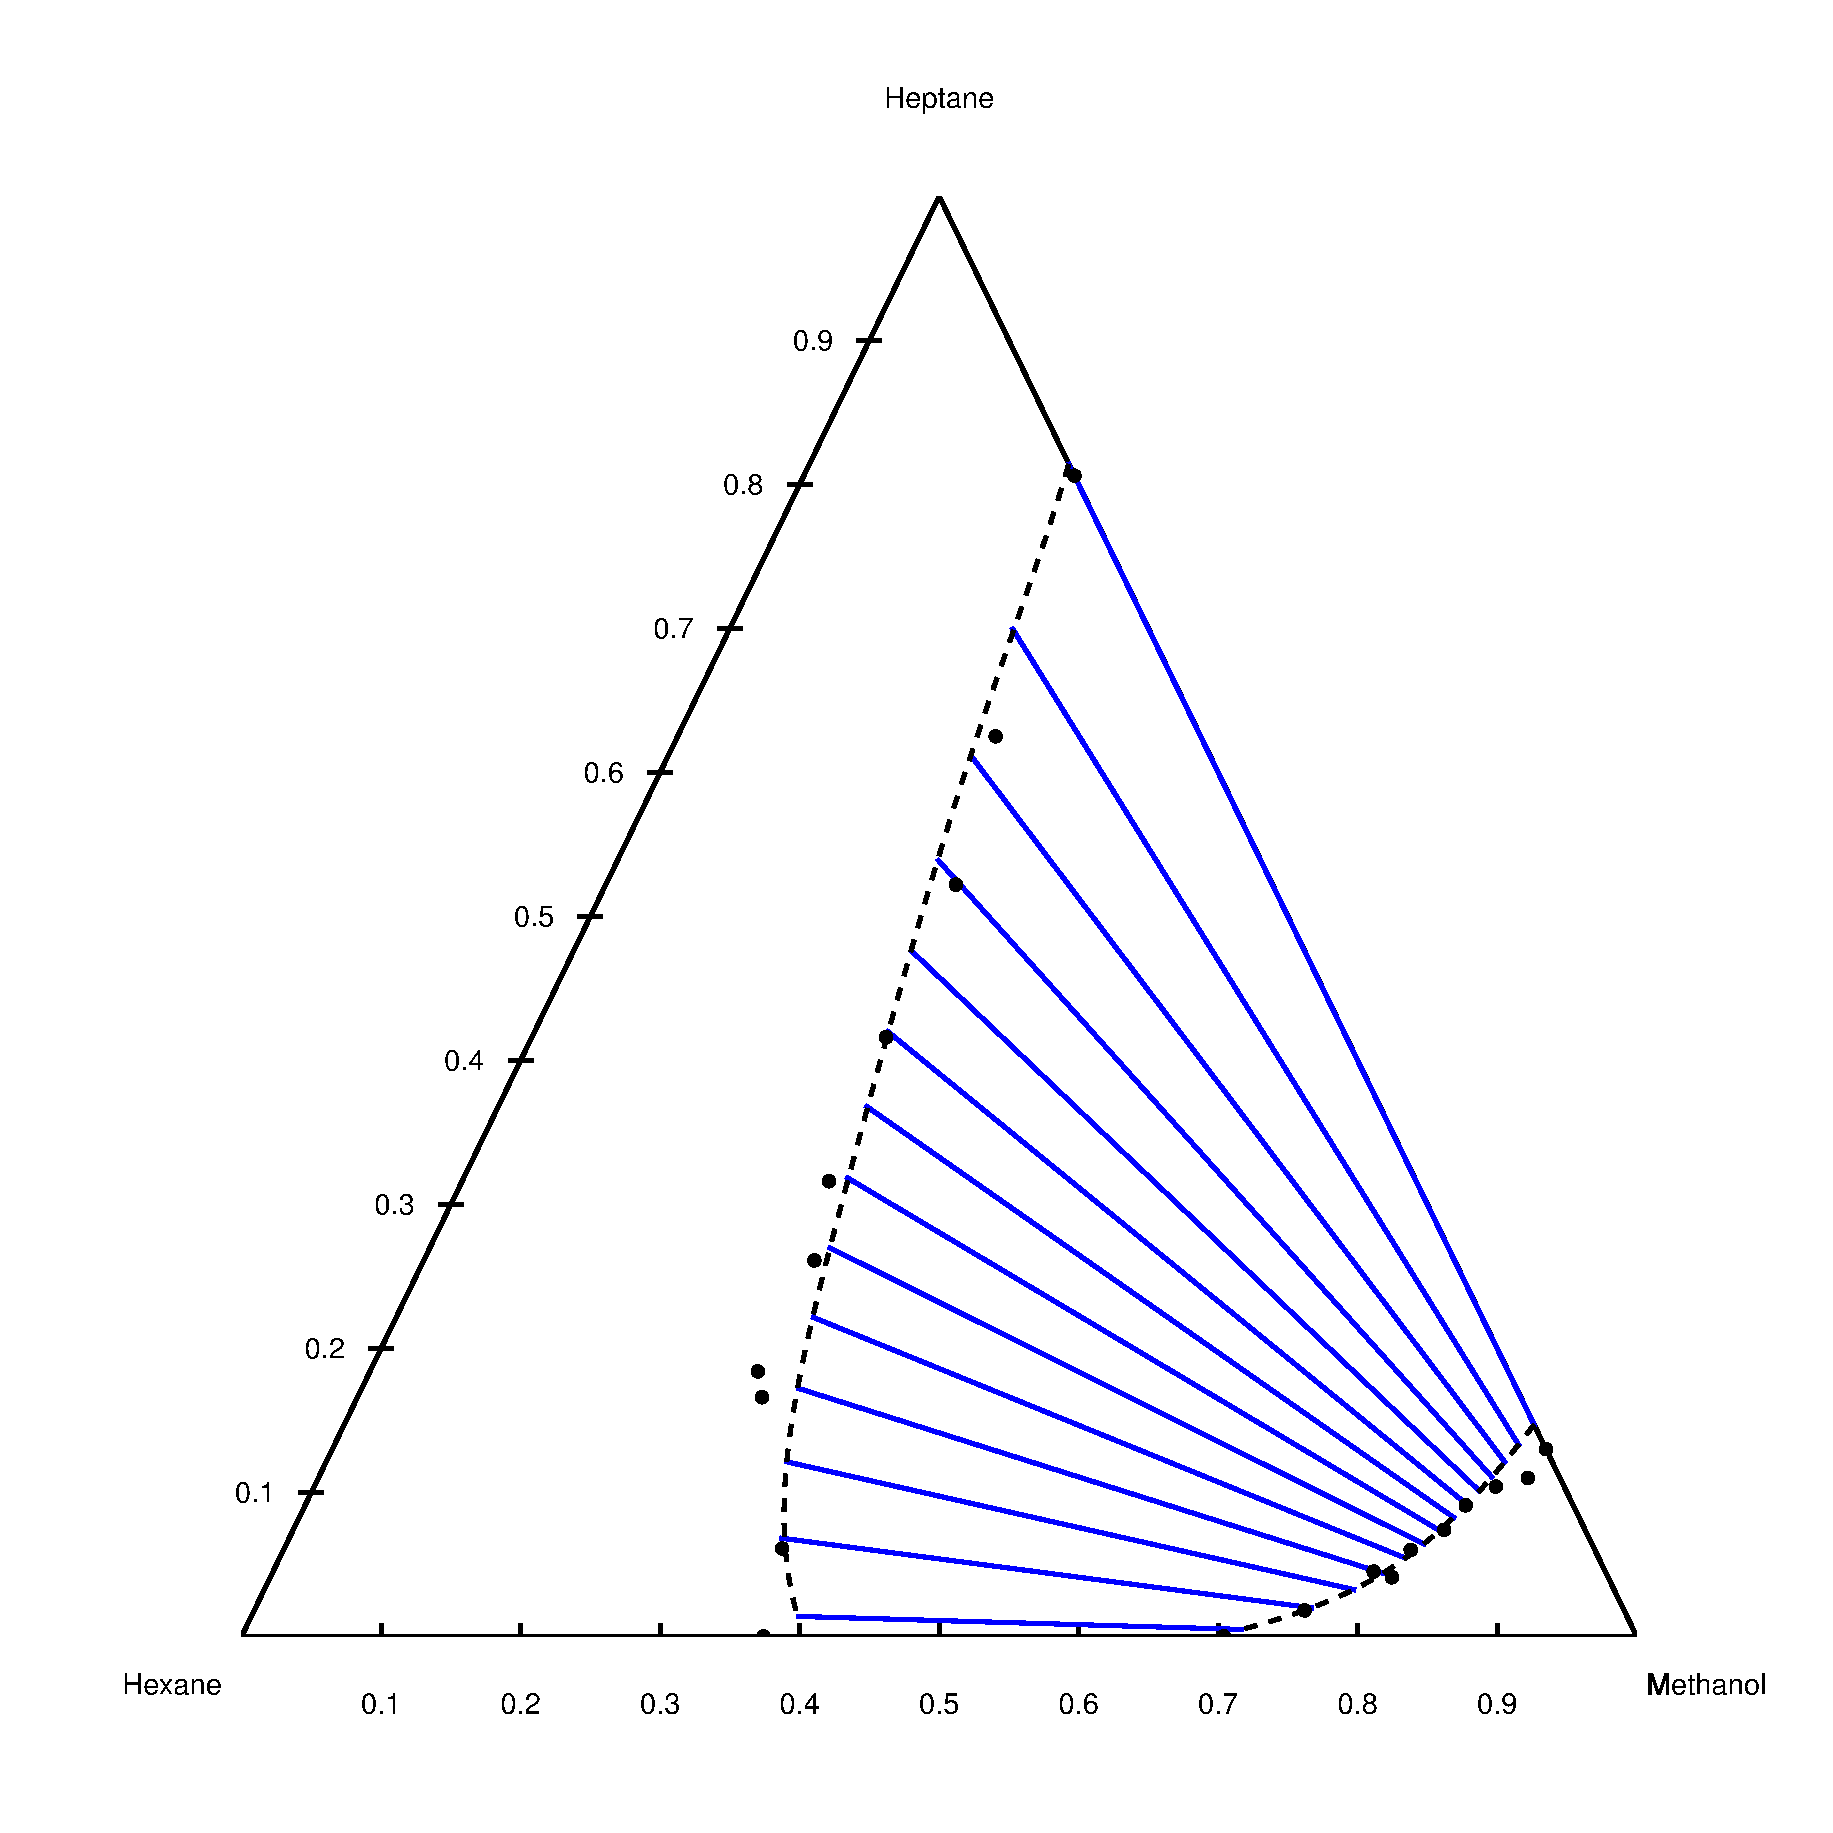
\includegraphics[width = 0.85\textwidth]{Results_Parts/TernaryParams/heptane-hexane-methanol/DWPMTieline3and-2/CalculatedPhaseDiagram.eps}
\caption{Calculated ternary phase diagram for Heptane, Hexane and Methanol, using the parameters calculated from the third and second last experimentally measured tielines} \label{heptane-hexane-methanolFigure2}
\end{figure}	
\clearpage

%%1-Hexanol-Methanenitro-Water-------------------------------------------------------------------------------------%

The parameter calculation for the system 1-Hexanol, Nitro-Methane and Water was performed at $294.15~\mathrm{K}$ and $296.15~\mathrm{K}$. At these temperatures three two-phase regions are observed. The experimentally measured tie-line compositions at $294.15~\mathrm{K}$ are given in table \ref{TielineData1-hexanol-methanenitro-water1}, and that at $296.15~\mathrm{K}$ in table \ref{TielineData1-hexanol-methanenitro-water2}.\\

Enforcing this behaviour during parameter estimation proved to be difficult and was not successful. The pseudo-analytical method used here utilises the information from two tie-lines. It is therefore not possible to enforce three two-phase regions simultaneously using the current approach. Predictably, by selecting both tie-lines for the parameter estimation from the same two-phase region, only that miscibility gap was accurately reproduced. The second and third two-phase regions were not predicted at all, and if they were it would have been coincidental. When forcing the model to match one tie-line each from two two-phase regions, the algorithm failed to converge to a viable solution.\\

The final output of the parameter estimation for the ternary mixture 1-Hexanol, Nitro-Methane and water is shown in table \ref{TernaryParameterResultsTable}. The corresponding Gibbs energy surfaces are given in figures \ref{1-hexanol-methanenitro-waterGibbsSurface1} and \ref{1-hexanol-methanenitro-waterGibbsSurface2}.\\

\begin{table}[hp]
\caption{Experimental tie-line data for the system 1-Hexanol, Nitro-Methane and Water at $294.15~\mathrm{K}$}
\begin{tabular}{cccccccccccc}
\toprule
\multicolumn{4}{c}{\textbf{Phase Split 1}} & \multicolumn{4}{c}{\textbf{Phase Split 2}} & \multicolumn{4}{c}{\textbf{Phase Split 3}}\\
\multicolumn{2}{c}{\textbf{Phase 1}} & \multicolumn{2}{c}{\textbf{Phase 2}} &\multicolumn{2}{c}{\textbf{Phase 1}} & \multicolumn{2}{c}{\textbf{Phase 2}} & \multicolumn{2}{c}{\textbf{Phase 1}} & \multicolumn{2}{c}{\textbf{Phase 2}}\\
$x_{1}$& $x_{2}$ &$x_{1}$& $x_{2}$ &$x_{1}$& $x_{2}$ &$x_{1}$& $x_{2}$ &$x_{1}$& $x_{2}$ &$x_{1}$& $x_{2}$ \\
\midrule
0.631 & 0.066& 0.001 & 0.015 & 0.183 & 0.620 &0.001 & 0.034& 0.296 & 0.446 & 0.183 & 0.620\\
0.528 & 0.154& 0.001 & 0.023 & 0.113 & 0.738 &0.001 & 0.034& 0.352 & 0.399 & 0.144 & 0.701\\
0.423 & 0.270& 0.001 & 0.028 & 0.070 & 0.814 &0.000 & 0.034& 0.410 & 0.364 & 0.128 & 0.744\\
0.296 & 0.446& 0.001 & 0.034 & 0.000 & 0.932 &0.000 & 0.034& 0.452 & 0.343 & 0.116 & 0.774\\
 & & & & & & & & 0.525 & 0.312 & 0.103 & 0.817\\
 & & & & & & & & 0.594 & 0.286 & 0.095 & 0.849\\
 & & & & & & & & 0.677 & 0.260 & 0.084 & 0.886\\
 & & & & & & & & 0.768 & 0.232 & 0.075 & 0.925\\
\bottomrule
\end{tabular}\\
\label{TielineData1-hexanol-methanenitro-water1}
\end{table}

\begin{table}[hp]
\caption{Experimental tie-line data for the system 1-Hexanol, Nitro-Methane and Water at $296.15~\mathrm{K}$}
\begin{tabular}{cccccccccccc}
\toprule
\multicolumn{4}{c}{\textbf{Phase Split 1}} & \multicolumn{4}{c}{\textbf{Phase Split 2}} & \multicolumn{4}{c}{\textbf{Phase Split 3}}\\
\multicolumn{2}{c}{\textbf{Phase 1}} & \multicolumn{2}{c}{\textbf{Phase 2}} &\multicolumn{2}{c}{\textbf{Phase 1}} & \multicolumn{2}{c}{\textbf{Phase 2}} & \multicolumn{2}{c}{\textbf{Phase 1}} & \multicolumn{2}{c}{\textbf{Phase 2}}\\
$x_{1}$& $x_{2}$ &$x_{1}$& $x_{2}$ &$x_{1}$& $x_{2}$ &$x_{1}$& $x_{2}$ &$x_{1}$& $x_{2}$ &$x_{1}$& $x_{2}$ \\
\midrule
0.622 & 0.070& 0.001 & 0.015 & 0.187 & 0.612 & 0.001 & 0.035& 0.179 & 0.675 & 0.355 & 0.440\\
0.527 & 0.153& 0.001 & 0.023 & 0.113 & 0.736 & 0.001 & 0.034& 0.150 & 0.730 & 0.407 & 0.400\\
0.422 & 0.268& 0.001 & 0.028 & 0.070 & 0.812 & 0.000 & 0.035& 0.125 & 0.792 & 0.499 & 0.346\\
0.256 & 0.502& 0.001 & 0.035 & 0.000 & 0.931 & 0.000 & 0.035& 0.111 & 0.830 & 0.570 & 0.313\\
 & & & & & & & & 0.096 & 0.877 & 0.652 & 0.285\\
 & & & & & & & & 0.082 & 0.918 & 0.736 & 0.264\\
\bottomrule
\end{tabular}\\
\label{TielineData1-hexanol-methanenitro-water2}
\end{table}

\begin{figure}[hp]
%\vspace{40pt}
\centering
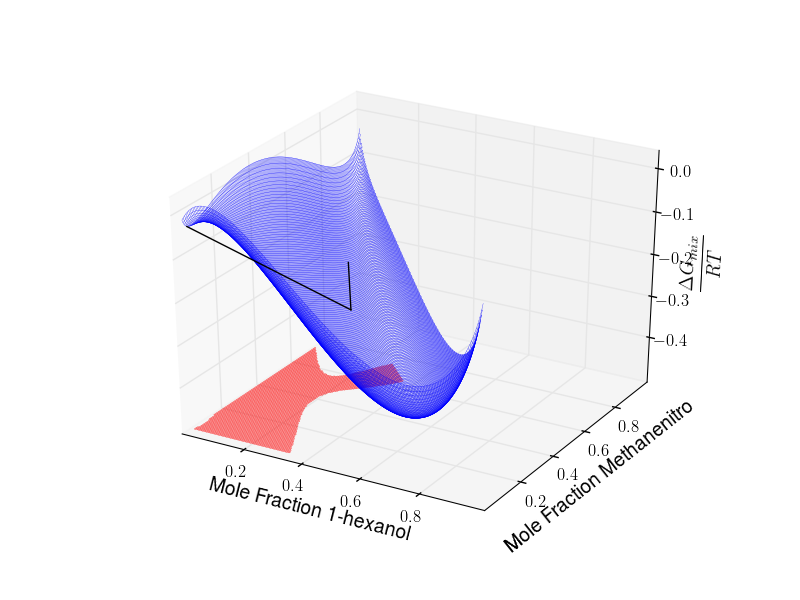
\includegraphics[width = 0.6\textwidth, bb=100 0 500 400]{Results_Parts/TernaryParams/1-hexanol-methanenitro-water/DWPM/294.15/PredictedGibbsWireframe.png}
\caption{Predicted Gibbs energy surface for 1-Hexanol, Nitro-Methane and Water at $294.15~\mathrm{K}$.}
\label{1-hexanol-methanenitro-waterGibbsSurface1}
\end{figure}	

\begin{figure}[hp]
%\vspace{40pt}
\centering
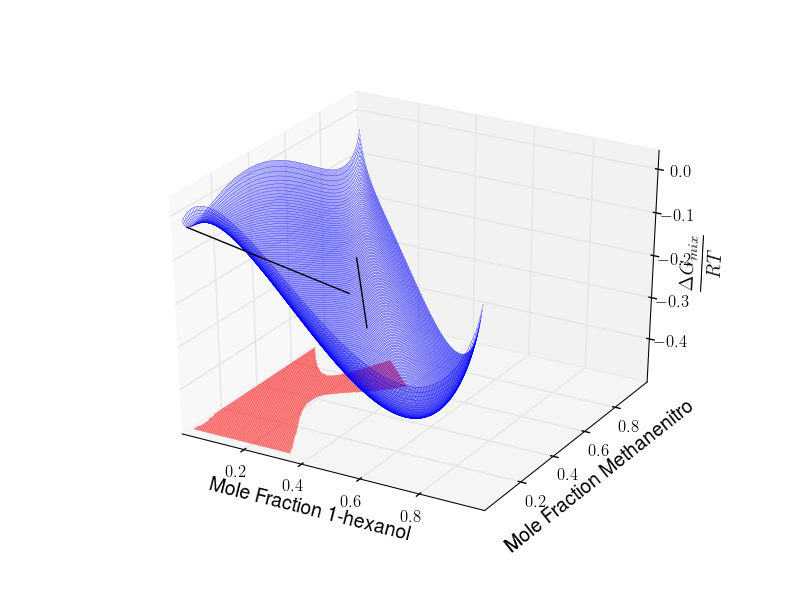
\includegraphics[width = 0.6\textwidth, bb=100 0 500 400]{Results_Parts/TernaryParams/1-hexanol-methanenitro-water/DWPM/296.15/PredictedGibbsWireframe.png}
\caption{Predicted Gibbs energy surface for 1-Hexanol, Nitro-Methane and Water at $296.15~\mathrm{K}$.}
\label{1-hexanol-methanenitro-waterGibbsSurface2}
\end{figure}
\clearpage

Similar to the case of binary mixtures, which may theoretically also exhibit multiple miscibility gaps, the thermodynamic behaviour exhibited by the system 1-Hexanol, Nitro-Methane and Water could possibly be better matched by allowing the $s_{i}$ parameters to be variable. The DWPM model possesses sufficient flexibility to accurately reproduce liquid-liquid equilibrium behaviour of ternary systems, which exhibit only one two-phase region, by varying the binary interaction parameters alone. For systems with more complex phase behaviour, instead of specifying each $s_{i}$, additional degrees of freedom may be built into the pseudo-analytical approach to better accommodate such behaviour.\\

For example, by using the equilibrium compositions from another tie-line, another six equilibrium relationships can be formulated and included in the set of equations to be solved. The six equations derived previously for each pair of tie-line compositions are given by:\

\begin{eqnarray}
g\left(x_{1}^{\alpha}, x_{2}^{\alpha}\right) = f_{j}\left(x_{1}^{\alpha}, x_{2}^{\alpha}\right) \\
g\left(x_{1}^{\beta}, x_{2}^{\beta}\right) = f_{j}\left(x_{1}^{\beta}, x_{2}^{\beta}\right)\\
\dfrac{\mathrm{d} g}{\mathrm{d}x_{1}}\left(x_{1}^{\alpha}, x_{2}^{\alpha}\right) = \dfrac{\mathrm{d} f_{j}}{\mathrm{d}x_{1}}\left(x_{1}^{\alpha}, x_{2}^{\alpha}\right)\\
\dfrac{\mathrm{d} g}{\mathrm{d}x_{1}}\left(x_{1}^{\beta}, x_{2}^{\beta}\right) = \dfrac{\mathrm{d} f_{j}}{\mathrm{d}x_{1}}\left(x_{1}^{\beta}, x_{2}^{\beta}\right)\\
\dfrac{\mathrm{d} g}{\mathrm{d}x_{2}}\left(x_{1}^{\alpha}, x_{2}^{\alpha}\right) = \dfrac{\mathrm{d} f_{j}}{\mathrm{d}x_{2}}\left(x_{1}^{\alpha}, x_{2}^{\alpha}\right)\\
\dfrac{\mathrm{d} g}{\mathrm{d}x_{2}}\left(x_{1}^{\beta}, x_{2}^{\beta}\right) = \dfrac{\mathrm{d} f_{j}}{\mathrm{d}x_{2}}\left(x_{1}^{\beta}, x_{2}^{\beta}\right)
\end{eqnarray}\

Where, as before, $x_{1}^{\alpha}$ and $x_{2}^{\alpha}$ are the compositions of components 1 and 2 in phase $\alpha$ respectively, and similarly $x_{1}^{\beta}$ and $x_{2}^{\beta}$ are the compositions of components 1 and 2 in phase $\beta$ respectively. And $f_{j}\left(x_{1}, x_{2}\right)$ is the common tangent plane $j$ to the Gibbs energy surface at both phase compositions:\

\begin{equation}
f_{j}\left(x_{1}, x_{2}\right) = a_{j}x_{1} + b_{j}x_{2} +c_{j} 
\end{equation}\

With the use therefore of the experimental data from three tie-lines, eighteen equations in total need to be solved. The variables to be solved for include $a_{j}$, $b_{j}$ and $c_{j}$ for each of the three tangent plane functions. The DWPM model parameters which are assumed to be unknown, are the six binary interaction parameters, and $s_{1}$ through $s_{3}$. Therefore, a total of eighteen unknown variables need to be calculated and the formulated system of equations is fully defined.\\

It is not known whether this system will have any solutions and if this approach will in-fact yield valid solutions to the parameter estimation problem. It, together with the choice of which tie-lines to use for the calculation, is left for future investigations.\\